\documentclass{PDS}

\usepackage{graphicx}
\usepackage{caption}
\usepackage{subcaption}

\usepackage{amsmath}
\usepackage{amssymb}
\usepackage{amsfonts}
\usepackage{amsthm}

\usepackage[round]{natbib}

\usepackage{newtxtext}
\usepackage{newtxmath}

\usepackage{xcolor}
\usepackage[colorlinks,allcolors=dscolor,bookmarks=false]{hyperref}

\jyear{2025}
\jdoi{https://doi.org/10.1017/pds.2025.xxx}

\begin{document}

\title{First experiences from using CADdrive with digital LEGO for product design and systems engineering education}

\author{Georg Hackenberg}
\author{Christian Zehetner}

\address{School of Engineering, University of Applied Sciences Upper Austria, 4600 Wels, Austria}

\corresemail{georg.hackenberg@fh-wels.at}

\abstract{
Due to rising product and system complexities, design and engineering have become a team effort that requires well planned and synchronized activities to achieve high degrees of process efficiency and effectiveness.
In recent years, online collaboration platforms emerged which help managing all relevant project information in a central repository and, hence, speed up the information flow between the different stakeholders.
However, inspiring high school children to pursue a carreer in this field and preparing undergraduate as well as graduate students for what they will face in practice remains a challenge for institutions and societies worldwide.
To overcome the current situation, in this paper we present our experiences with conducting different course formats both with children from high school as well as with adults pursueing a Master-level study programme.
We provide insights into the organization of the different course formats, the various backgrounds and profiles of their participants, the work results produced by the individual teams, as well as the participants' feedback.
Overall, we conclude that online collaboration platforms like CADdrive with integrated version management, issue tracking, and task scheduling are well suited for conducting project-based courses with predefined design tasks.
In particular, our participants appreciated the transparency which can be achieved by means of online collaboration platforms as well as the accountability of the individual team members, which fosters active participation and learning.
}

\keywords{product design, systems engineering, engineering education}

\maketitle

\section{Introduction}
\label{sec:introduction}

\cite{Luo_2017} show based on U.S.\ patent data that the complexity of innovation processes and their outcomes has been growing steadily over the past 20 years.
According to \cite{Trattner_2019} the growing complexity of our products and systems can be seen, for example, in the growing number of components, their interfaces, and their interactions.
Futhermore, \cite{Thramboulidis_2008} explains that the interfaces between these components typically are not limited to one engineering discipline (e.g.\ mechanics or electrics) anymore, but span several disciplines.
Ultimately, we deal with a mutlitude of mechatronic components, which exhibit relevant mechanical, electrical, and logical characteristics.
For such mechatronic components, \cite{Youcef_Toumi_1996} already identified that they come with their own integration issues, which are not considered in the classical engineering disciplines.

In the past, the sole ability to engineer such complex systems might have been a sufficient success factor for societies and organizations.
As \cite{Senescu_2014} argue, today due to rising global competition in many domains the engineering ability alone is not sufficient anymore, but the efficiency and effectiveness of the underlying engineering processes must be considered.
According to \cite{Zidane2017}, different definitions exist for the terms \textit{efficiency} and \textit{effectiveness} in this context.
One possible definition of efficiency is that the overall engineering process can be executed as fast as possbile and the desired target system's time-to-market is minimized.
In contrast, one possible definition of effectiveness is that the engineering process leading to the desired target system consumes as little resources as possible and, hence, the overall process costs are minimized.

As \cite{Strauss_1985} already argued, one key to efficiency (i.e.\ high development speeds) is dividing the overall work into individual activities, which can be executed in parallel, but also might require synchronization of their work results.
\cite{Hartmann_2022} explain that these activities must be scheduled carefully such that the work results of one activity are ready when they are needed by another acitivity, leading to the well-known project scheduling problem.
When required work results are not ready in time, you typically have two choices:
Either you delay follow-up activities potentially causing a suboptimal utilization of project resources as \cite{Kumaraswamy_1998} explain for the construction industry.
Or you start follow-up activities anyways and risk working with wrong assumptions causing unnecessary revisions of work results later in the process as \cite{Chapman_2006} argues from the viewpoint of project and risk management.

In contrast, \cite{Maalem_2016} argue that one key to effectiveness is to understand stakeholder requirements and validate assumptions as early as possible in the engineering process.
According to \cite{Mobin_2019} validation activities must be planned where applicable to ensure that such mistakes are uncovered and resolved quickly and to minimize their impact on the future course of the project.
In this context, agile methodologies and frameworks have emerged over the past two decades ensuring stakeholder integration along the entire development process as \cite{Chan_2009} explain.
In agile approaches, stakeholders have the obligation to review work results frequently and give their feedback to engineering team as \cite{Deininger_2019} describe.

Furthermore, \cite{Hackenberg_2023} argue that online collaboration platforms with vision management, issue tracking, and task scheduling support engineering teams in achieving high degrees of efficiency and effectiveness.
\cite{Tony_Liu_2001} already explained that the idea behind such web-based platforms is to bundle all relevant project information in a central repository, to which all stakeholders have access from anywhere, anytime, and with any device.
And \cite{Kraemer_1988} already noted that online collaboration platforms can improve the speed of information flow between the stakeholders significantly compared to traditional approaches.
Higher speeds of information flow, in turn, reduce the risk of project delays as well as incorrect assumptions and unnecessary revisions of work results as \cite{Novak_2009} show, e.g., in the food industry.

Now, as academic teachers we try to prepare our students as good as possible for what they will face in practice.
Ideally, our graduates quickly find their place in multi-disciplinary engineering teams and contribute reliably to the success of their projects.
However, beyond the core technical skills they need a solid understanding of the overall engineering processes, the overarching efficiency and effectiveness objectives, as well as the employed collaboration principles as \cite{Deshpande_2011} argue.
According to \cite{Meyer_2020} teaching such profound understanding of process, team, and collaboration dynamics still remains a major challenge for engineering education.

\paragraph{Research question}

To overcome the current situation in engineering education, we wanted to understand how well different course formats and settings work based on a representative online collaboration platform and the digital LEGO framework.
In particular, we wanted to understand the suitability of different course formats as well as the underlying platform and framework for Master-level product design and systems engineering education.
Furthermore, we were interested in how well such course formats work for children from high school aged between 10 and 15 years old, how well they can deal with CAD programs, and how well they understand the inherent collaboration challenges.

\paragraph{Contribution}

To answer the previous research questions, we conducted two Master-level courses on product design and systems engineering as well as one workshop with high school children.
The organizational structure of the two Master-level courses as well as the workshop, and the work results of the different teams are explained in Section~\ref{sec:contribution}.
During and after conducting the experiments we collected feedback from the individual participants and analyzed the data as discussed in Section~\ref{sec:discussion}.
Finally, we draw our conclusions from the previous experiments and their data, derive our key learnings, and sketch out important future work towards high impact engineering education in Section~\ref{sec:conclusion}.

\section{Course experiments}
\label{sec:contribution}

For our experiements we used the open source software CADdrive\footnote{\url{https://github.com/ghackenberg/caddrive}} as the underlying online collaboration platform with version management, issue tracking, and task scheduling, as well as the open source software LeoCAD\footnote{\url{https://github.com/leozide/leocad}} for digital LEGO design.
% and  Dassault Systèmes SolidWorks\footnote{\url{https://www.solidworks.com/}} for classical CAD.
Subsequently, we first describe our Master-level course formats with students at University of Applied Sciences Upper Austria in Section~\ref{sec:master}, before explaining our workshop format with high school children in Section~\ref{sec:school}.
Both for the Master-level courses and the workshop we introduce the organizational settings and show the most interesting work results delivered by the individual teams.

\subsection{Master level}
\label{sec:master}

At Master level, we conducted two courses with about 30 work hours per student in two independent study programmes with slightly varied study plans and, hence, organizational settings.
The goal of the first course was to design a energy-optimal glasshouse for growing sweet tomatos over the winter months in Alpine regions as explained in Section~\ref{sec:master-product-lego}.
Furthermore, the course included a fair amount of simulation tasks for verification and validation.
The goal of the second course was to design a paper folding machine turning plain paper sheets into boxes as expained in Section~\ref{sec:master-system-lego}.
However, the course did not include simulation tasks, but verification and validation was achieved through manual reviews only.
%And the goal of the thrid course was to design two innovative, but not otherwise constrained products in the vertical farming space as explained in Section~\ref{sec:master-product-classical}.

\subsubsection{Glasshouse for Alpine regions}
\label{sec:master-product-lego}

The first course started in the winter term 2023 in the full-time Master programme "Innovation and Product Management".
The participants included 5 women and 5 men between 26 and 40 years old having between 1 and 16 years of work experience in different industries (e.g.\ automotive, retail, banking, etc.) and departments (e.g.\ product development, logistics, martketng and sales, etc.).
Furthermore, 8 students were holding a Bachelor degree and 2 students were holding a Master degree in some field.
Also, most students were already familiar with some CAD tool (e.g.\ PTC Creo, AutoDesk AutoCAD, Siemens NX, etc.) as well as simulation software (e.g.\ Abaqus, Matlab Simulink, Ansys, etc.).

In this project-based course, the goal of the group was to design an energy-efficient glasshouse for growing sweet tomatos over the winter months in Alpine regions.
The tasks included requirements analysis, modular architecture design, mechanical design, electrical design, and simulation-based verification of selected system properties.
Figure~\ref{fig:glasshouse} shows the mechanical design developed by the group with digital LEGO bricks and LeoCAD.
The mechanical design comprises a grow area for the plants with glass walls and windows as well as solar panels on the roof (see Figure~\ref{fig:glasshouse_2}), and a shed area for storing tools and batteries (see Figure~\ref{fig:glasshouse_3}).

\begin{figure}[htbp]
    \begin{subfigure}[b]{0.32\textwidth}
        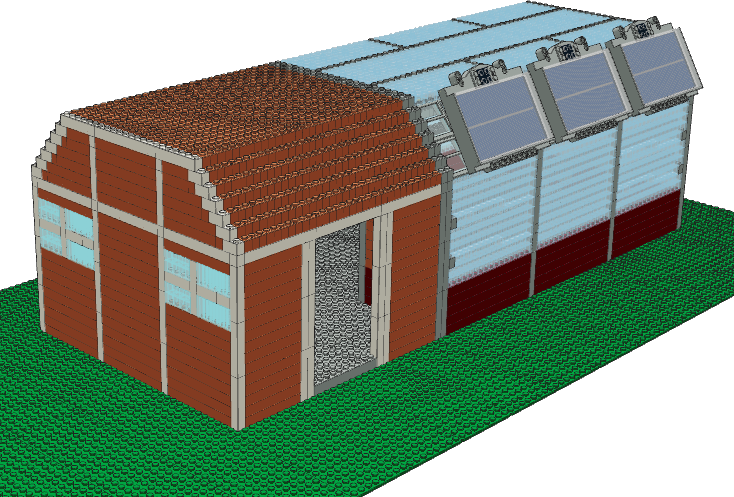
\includegraphics[width=\textwidth]{./figures/glasshouse_1.png}
        \caption{Exterior design}
        \label{fig:glasshouse_1}
    \end{subfigure}
    \hfill
    \begin{subfigure}[b]{0.32\textwidth}
        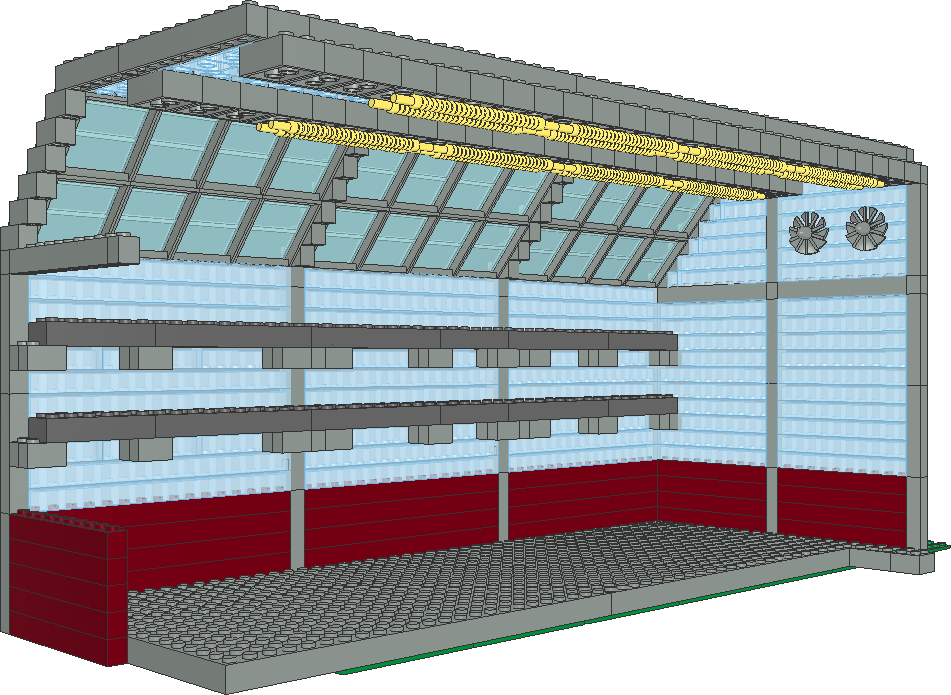
\includegraphics[width=\textwidth]{./figures/glasshouse_2.png}
        \caption{Interior design (grow area)}
        \label{fig:glasshouse_2}
    \end{subfigure}
    \hfill
    \begin{subfigure}[b]{0.32\textwidth}
        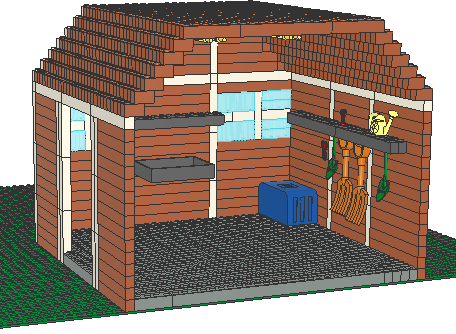
\includegraphics[width=\textwidth]{./figures/glasshouse_3.png}
        \caption{Interior design (shed area)}
        \label{fig:glasshouse_3}
    \end{subfigure}
    \caption{Mechanical design of the glasshouse with digital LEGO bricks.}
    \label{fig:glasshouse}
\end{figure}

In the context of simulation-based verification, the group was tasked with applying finite element analysis (FEA), computational fluid dynamics (CFD), and multi-physics simulation (MPS) for analyzing selected system properties.
The group decided to apply finite element analysis for analyzing the stability of the mechanical structure under snow and wind pressure, as well as computational fluid dynamics for analyzing the heat loss characteristics of the building.
Furthermore, the group decided to employ multi-physics simulation with OpenModelica\footnote{\url{https://github.com/OpenModelica/OpenModelica}} for analyzing the electrical energy consumption caused by the automatic window opening and closing system as shown in Figure~\ref{fig:glasshouse-sim}.

\begin{figure}[htbp]
    \begin{subfigure}[b]{0.575\textwidth}
        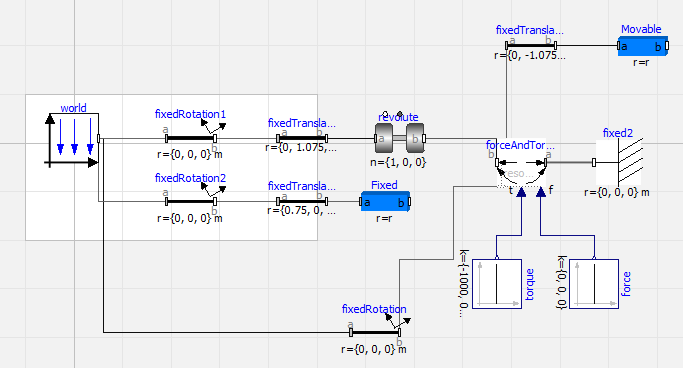
\includegraphics[width=\textwidth]{./figures/glasshouse_mechatronic_1.png}
        \caption{OpenModelica component model}
        \label{fig:glasshouse-sim-1}
    \end{subfigure}
    \hfill
    \begin{subfigure}[b]{0.41\textwidth}
        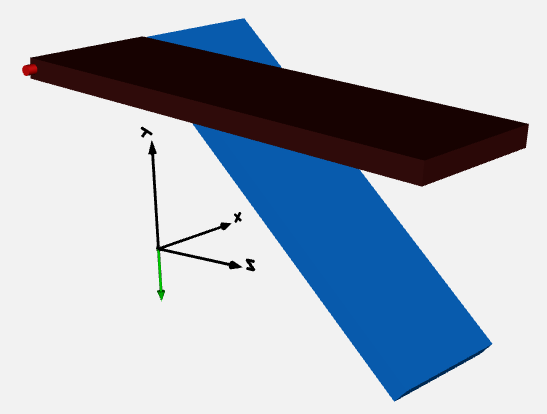
\includegraphics[width=\textwidth]{./figures/glasshouse_mechatronic_2.png}
        \caption{OpenModelica 3D visualization}
        \label{fig:glasshouse-sim-2}
    \end{subfigure}
    \caption{Multi-physics simulation of automatic window opening and closing system.}
    \label{fig:glasshouse-sim}
\end{figure}

% TODO

\subsubsection{Paper folding machines}
\label{sec:master-system-lego}

The second course also started in the winter term 2023 in the part-time Master programme "Robotic Systems Engineering".
The participants included 1 woman and 12 men between 25 and 33 years old having between 3 and 10 years of work experience in different industries (e.g.\ logistics, chemical, agriculture, etc.) and departmets (e.g.\ automation engineering, business development, project management, etc.).
Furthermore, all students were holding a Bachelor degree in some technical field.
Also, most students were familar with some CAD software (e.g.\ AutoDesk AutoCAD, Dassault Systèmes Catia, PTC Creo, etc.), while only two students did not have prior CAD experience.

The course was divided into two parts, a theory part followed by a practice part.
In the theory part different concepts such as systems engineering, systems lifecycle processes, requirements analysis, systems architecture, systems integration, as well as verification and validation were introduced.
In the practice part the students were split into teams and were given the goal of developing a paper folding machine, which turns plain paper sheets into boxes with defined measures.
The tasks included requirements analysis, mechatronic systems architecture derivation, as well as mechanical, electrical, and logical system design.
Figure~\ref{fig:paper} shows three different mechanical designs proposed by the teams.

\begin{figure}[htbp]
    \begin{subfigure}[b]{0.32\textwidth}
        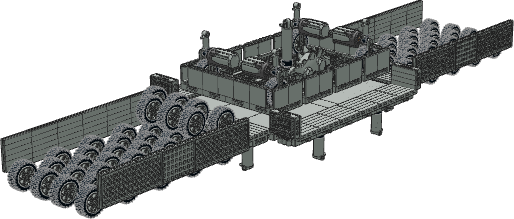
\includegraphics[width=\textwidth]{./figures/paper_1.png}
        \caption{First team}
        \label{fig:paper_1}
    \end{subfigure}
    \hfill
    \begin{subfigure}[b]{0.32\textwidth}
        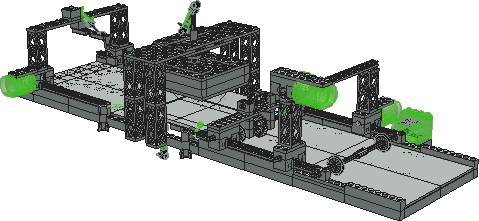
\includegraphics[width=\textwidth]{./figures/paper_2.png}
        \caption{Second team}
        \label{fig:paper_2}
    \end{subfigure}
    \hfill
    \begin{subfigure}[b]{0.32\textwidth}
        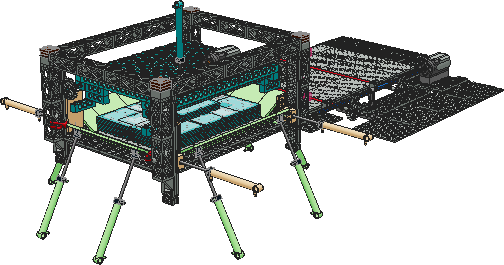
\includegraphics[width=\textwidth]{./figures/paper_3.png}
        \caption{Third team}
        \label{fig:paper_3}
    \end{subfigure}
    \caption{Different mechanical designs of the paper folding machine.}
    \label{fig:paper}
\end{figure}

In contrast, Figure~\ref{fig:paper-sub} shows the electrical and logical design of one paper folding machine.
This particular team worked with EPLAN Electric P8\footnote{\url{https://www.eplan-software.com/solutions/eplan-electric-p8/}} for the electrical design as well as Excalidraw\footnote{\url{https://excalidraw.com/}} for the logical design of the target system.
Note that in this case one student was already familiar with EPLAN Electric P8, which is why the first tool was selected.
Furhtermore, note that the notation for the logical design was not prescribed by the course instructor, but resembles some form of state chart formalism, which is common in control engineering.
Finally, validation of the different designs was performed with manual review techniques across all teams.

\begin{figure}[htbp]
    \centering
    \begin{subfigure}[b]{0.45\textwidth}
        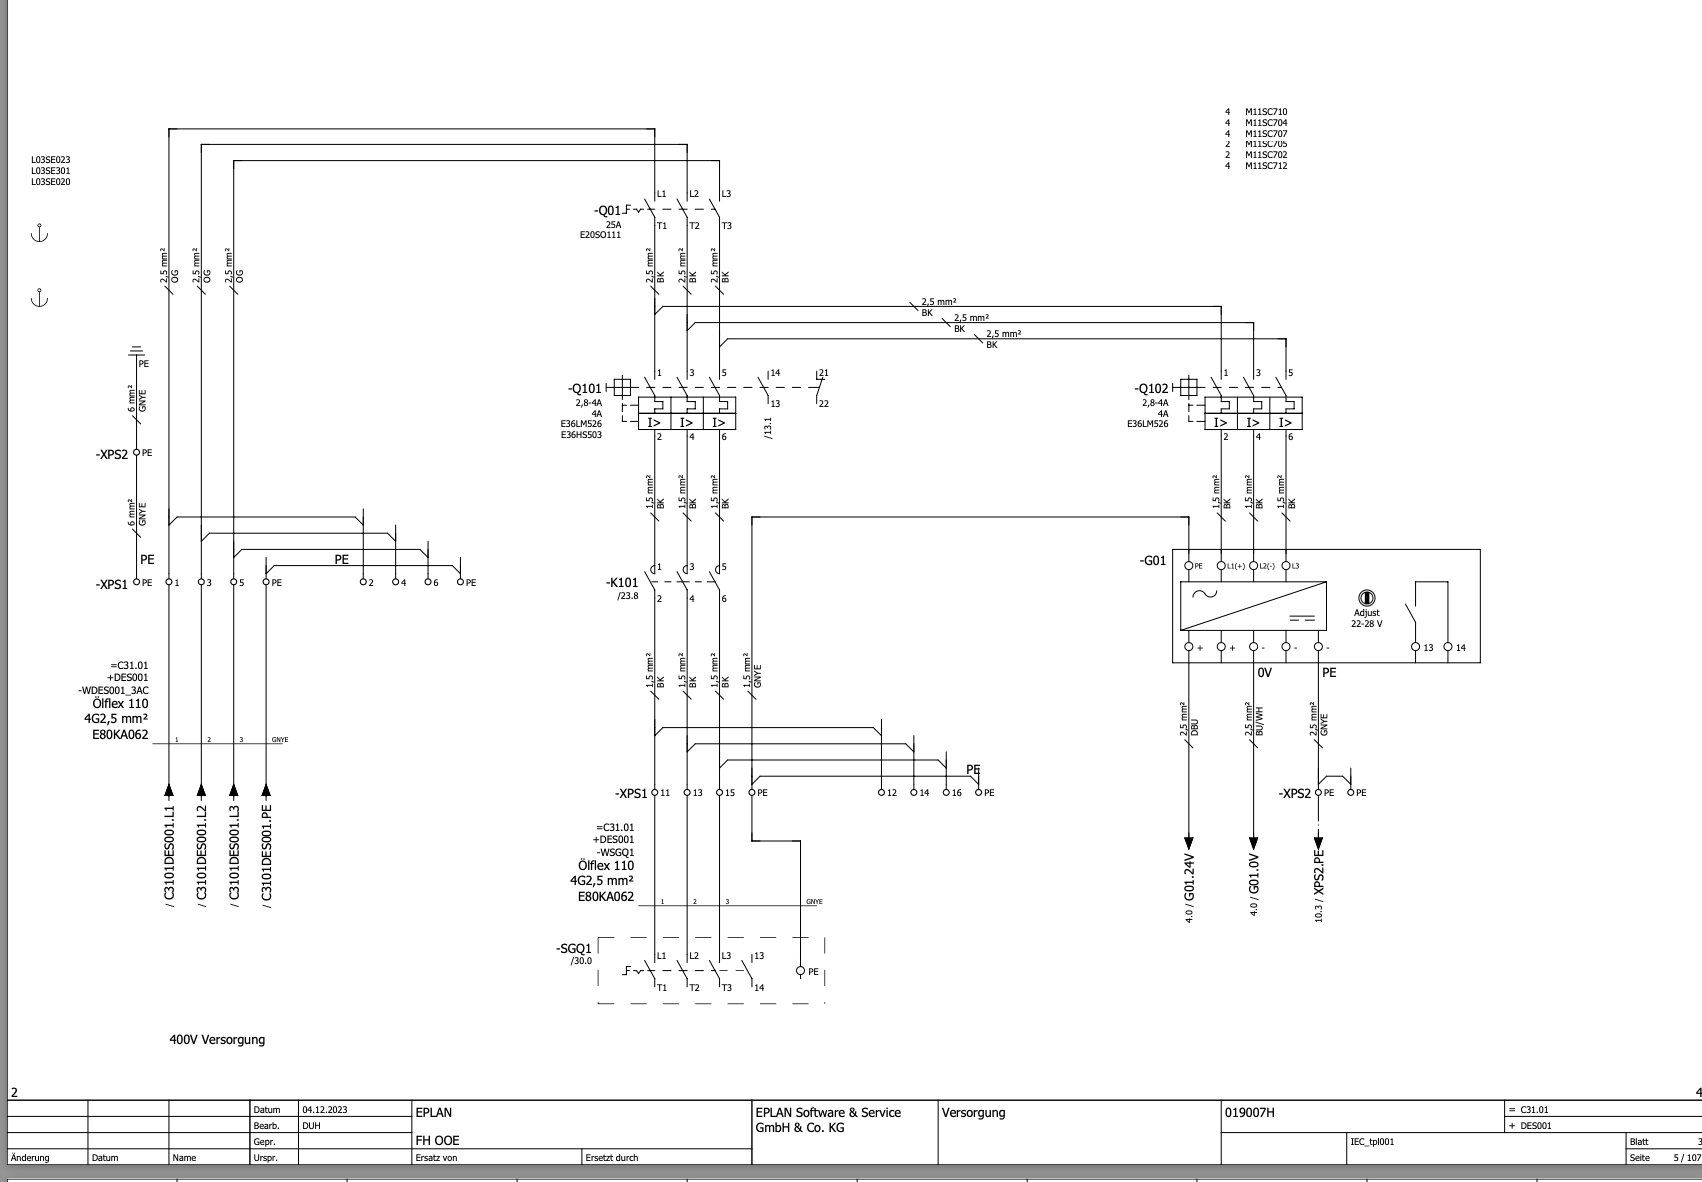
\includegraphics[width=\textwidth]{./figures/paper_electric.png}
        \caption{Electrical design}
        \label{fig:paper-sub-1}
    \end{subfigure}
    \hfill
    \begin{subfigure}[b]{0.5\textwidth}
        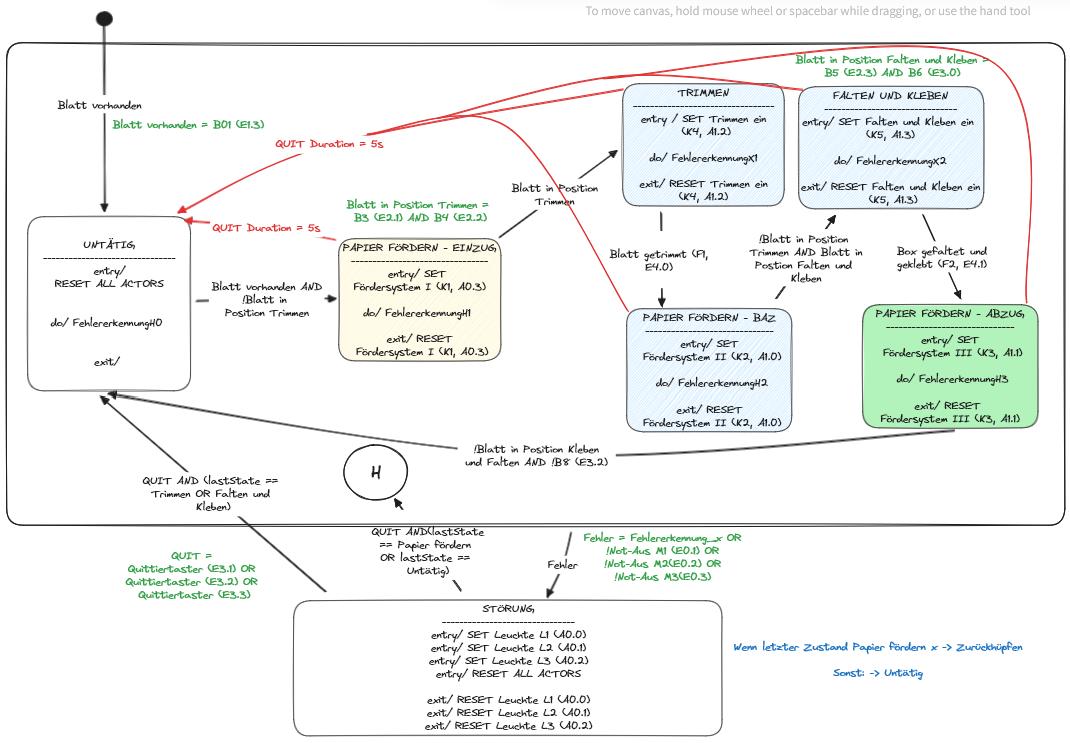
\includegraphics[width=\textwidth]{./figures/paper_control.png}
        \caption{Logical design}
        \label{fig:paper-sub-2}
    \end{subfigure}
    \caption{Electrical and logical design of one paper folding machine.}
    \label{fig:paper-sub}
\end{figure}

\subsection{High school level}
\label{sec:school}

At high school level, we conducted one single-day workshop with children from around Wels city in Upper Austria.
The workshop was organized as part of the KinderUni\footnote{\url{https://www.kinderuni-ooe.at/}} summer programme at the the School of Engineering of the University of Applied Sciences of Upper Austria in Wels, Austria.
The KinderUni programme provides children the chance to experience science hands-on and to learn about different topics such as engineering, biology, architecture, and many more.
Section~\ref{sec:school-lego} explains the structure of this single-day workshop and highlights results developed by the children during the course of the workshop.

\subsubsection{LEGO product ideas}
\label{sec:school-lego}

The workshop took place in July 2024 and was organized by the Upper Austrian branch of the KinderUni in Wels city\footnote{\url{https://www.kinderuni-ooe.at/kinderuni-ooe/wels/}}.
The workshop participants included 7 girls and 12 boys between 10 and 15 years old from different primary and high schools in the region, some -- but not all -- knowing each other from the same school.
In the morning, the children were brought to the School of Engineering of the University of Applied Sciences Upper Austria by their parents and were welcomed by an official representative of KinderUni.
The workshop itself lasted from morning until late afternoon and included short breaks before and after noon as well as a lunch break.

During the workshop, the hosts first presented the workshop agenda and the goal of the design projects before explaining and demonstrating the basics of LeoCAD for digital LEGO design.
Then the children were divided into teams of two with one girl working alone due to the uneven number of workshop participants.
The goal of each team was to develop an idea for a new LEGO product, while the target group (e.g.\ male or female), the target age (e.g.\ under 10, under 16, over 18, etc.), and the target theme (e.g.\ science fiction, princess, holiday, etc.) for the product could be selected freely.
Figure~\ref{fig:kinderuni} shows three product designs, which have been proposed by the teams.

\begin{figure}[htbp]
    \centering
    \begin{subfigure}[b]{0.3\textwidth}
        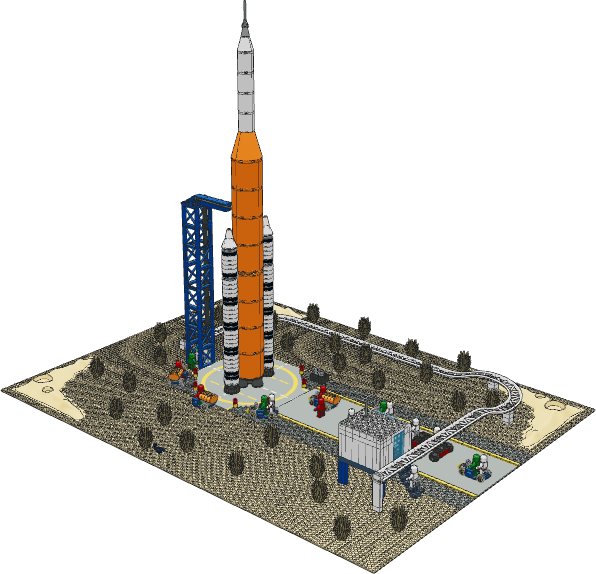
\includegraphics[width=\textwidth]{./figures/space.png}
        \caption{Space station}
        \label{fig:rocket}
    \end{subfigure}
    \hfill
    \begin{subfigure}[b]{0.3\textwidth}
        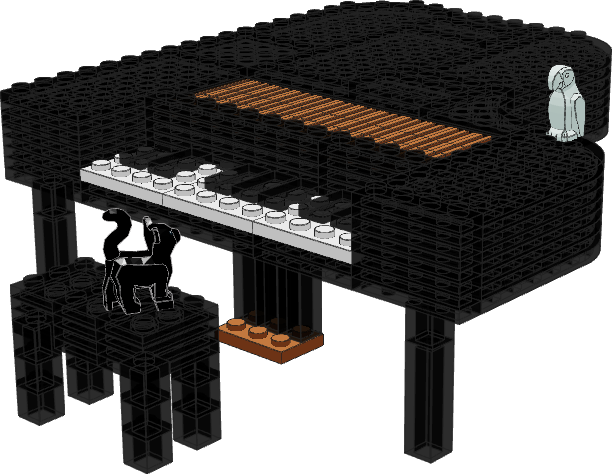
\includegraphics[width=\textwidth]{./figures/piano.png}
        \caption{Animal piano}
        \label{fig:piano}
    \end{subfigure}
    \hfill
    \begin{subfigure}[b]{0.3\textwidth}
        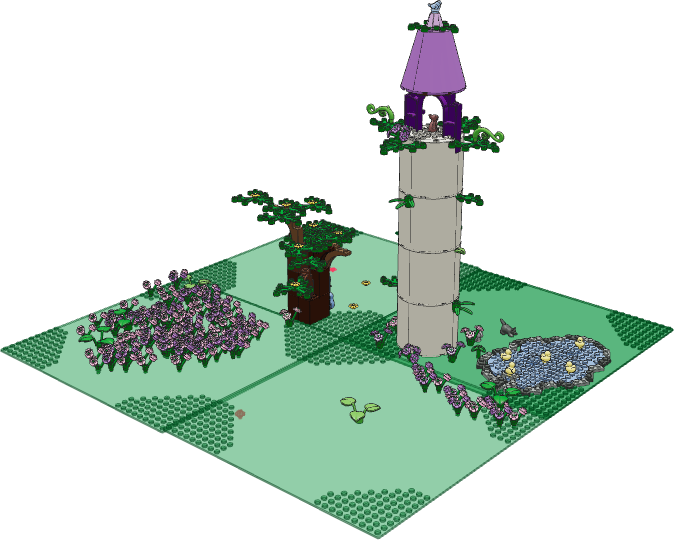
\includegraphics[width=\textwidth]{./figures/rapunzel.png}
        \caption{Rapunzel tower}
        \label{fig:rapunzel}
    \end{subfigure}
    \caption{LEGO product designs proposed by the teams during the workshop.}
    \label{fig:kinderuni}
\end{figure}

For all teams, one requirement was that they uploaded the current state of their digital LEGO designs every hour to CADdrive, so that the design process can be reconstructed and visualized.
For teams including two members, another challenge was dividing their work into two independent modules, developing the two modules separately, and integrating the modules at the end of the workshop day.
Three out of nine two-member teams managed to master this challenge (as, e.g., shown in Figure~\ref{fig:school-sub}), while three two-member teams decided not to divide their work, but decided to work together in front of one computer only.
The remaining three two-member teams failed integrating their work.

\begin{figure}[htbp]
    \centering
    \begin{subfigure}[b]{0.25\textwidth}
        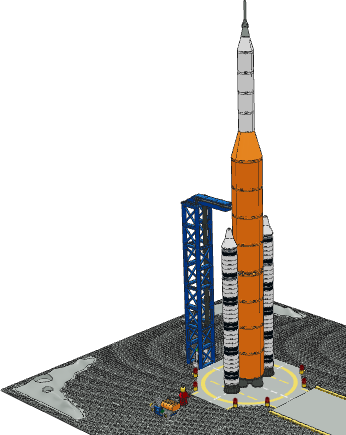
\includegraphics[width=\textwidth]{./figures/space_rocket.png}
        \caption{Rocket component}
    \end{subfigure}
    \hfill
    \begin{subfigure}[b]{0.45\textwidth}
        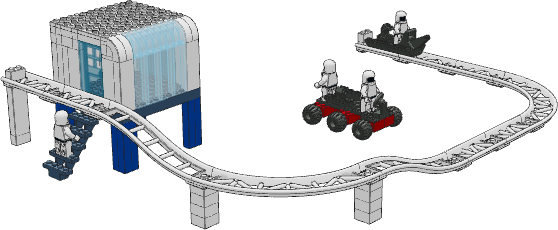
\includegraphics[width=\textwidth]{./figures/space_station.png}
        \caption{Station component}
    \end{subfigure}
    \hfill
    \begin{subfigure}[b]{0.25\textwidth}
        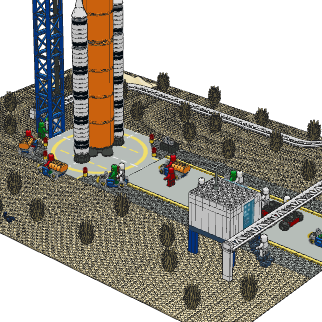
\includegraphics[width=\textwidth]{./figures/space_assembly.png}
        \caption{Component assembly}
    \end{subfigure}
    \caption{Components of the space station LEGO product idea and their assembly.}
    \label{fig:school-sub}
\end{figure}

\section{Evaluation results}
\label{sec:discussion}

After conducting the experiments from the previous section, we performed a systematic evaluation on the Master-level courses as well as an informal feedback round on the workshop to understand the current quality of our educational offering.
For systematic evaluation, we developed a questionnaire assessing the prior experience of the course participants in different knowledge domains as well as the learning experience during the course.
Note that there were some differences between the questionnaires of the two Master-level courses, which is why not all quantitative results add up to the total number of participants (i.e.\ 24 students).
In the following, we first present the results of the assessment of prior expierience in Section~\ref{sec:prior} before going into the details of the assessment of the learning experience in Section~\ref{sec:learning}.

\subsection{Prior experience}
\label{sec:prior}

Figure~\ref{fig:before} summarizes the results of the assessment of prior experiences of our Master-level course participants.
In our questionnaire we assessed prior experiences in different fields such as CAD/CAM (\textit{medium}), simulation (i.e.\ FEM/CFD/MBS/MPS/DES; \textit{low}), PDM/PLM (\textit{high}), QFD/DSM (\textit{low}), product management/design (\textit{medium}), systems/requirements/mechanical/electrical/software engineering (\textit{high}), as well as project management, agile methodology, and design thinking (\textit{high}).
Note that in each category the participants selected between novice, junior, professional, senior, and expert experience levels, which we aggregated to low, medium, and high levels here for gaining a bigger picture.

\begin{figure}[htbp]
    \centering
    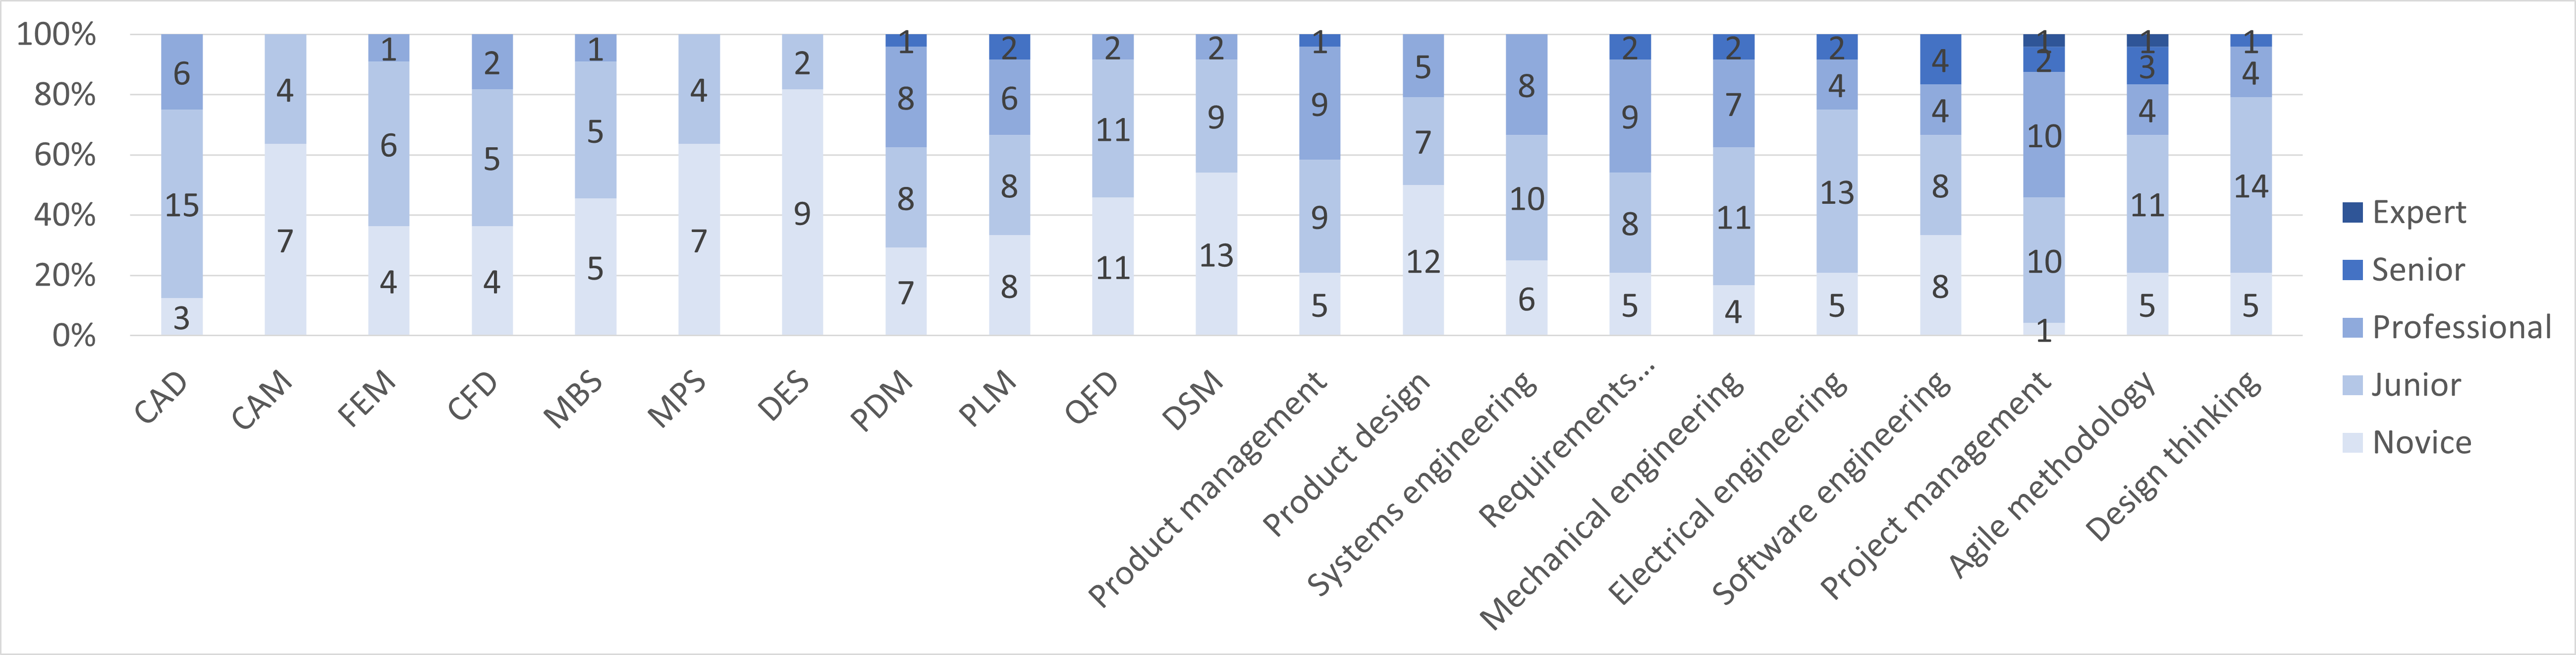
\includegraphics[width=\textwidth]{./diagrams/before.png}
    \caption{Summary of prior experience in different knowledge areas.}
    \label{fig:before}
\end{figure}

\subsection{Learning experience}
\label{sec:learning}

For assessing the learning experience during the two Master-level courses on product design and systems engineering, the questionnaire included a quantitative and a qualitative section.
In the quantitative section we assessed the general learning experience, the learning experience in different knowledge areas (e.g.\ digital collaboration and agile methodology), and the learning experience with the different software tools (e.g.\ CADdrive and LeoCAD) as described in Section~\ref{sec:quantitative}.
In the qualitative section we asked the participants about ideas for improvement of the two different course concepts as well as the software tools employed as described in Section~\ref{sec:qualitative}.

\subsubsection{Quantitative feedback}
\label{sec:quantitative}

Figure~\ref{fig:after-general} summarizes the results of the assessment of the general learning experience during the courses.
In this section of the questionnaire, we assessed the overall experience, the study programme relevance, the study programme integration, the course concept, the course organization, the motivation level, the activation level, the LEGO framework, and the use case.
As one can see, the tendency among all factors is positive with overall experience, study programme relevance, course concept, and use case rated among the best.
On the other hand, one can see that the study programme integration, the course organization, and the digital LEGO framework show potential for improvement.

\begin{figure}[htbp]
    \centering
    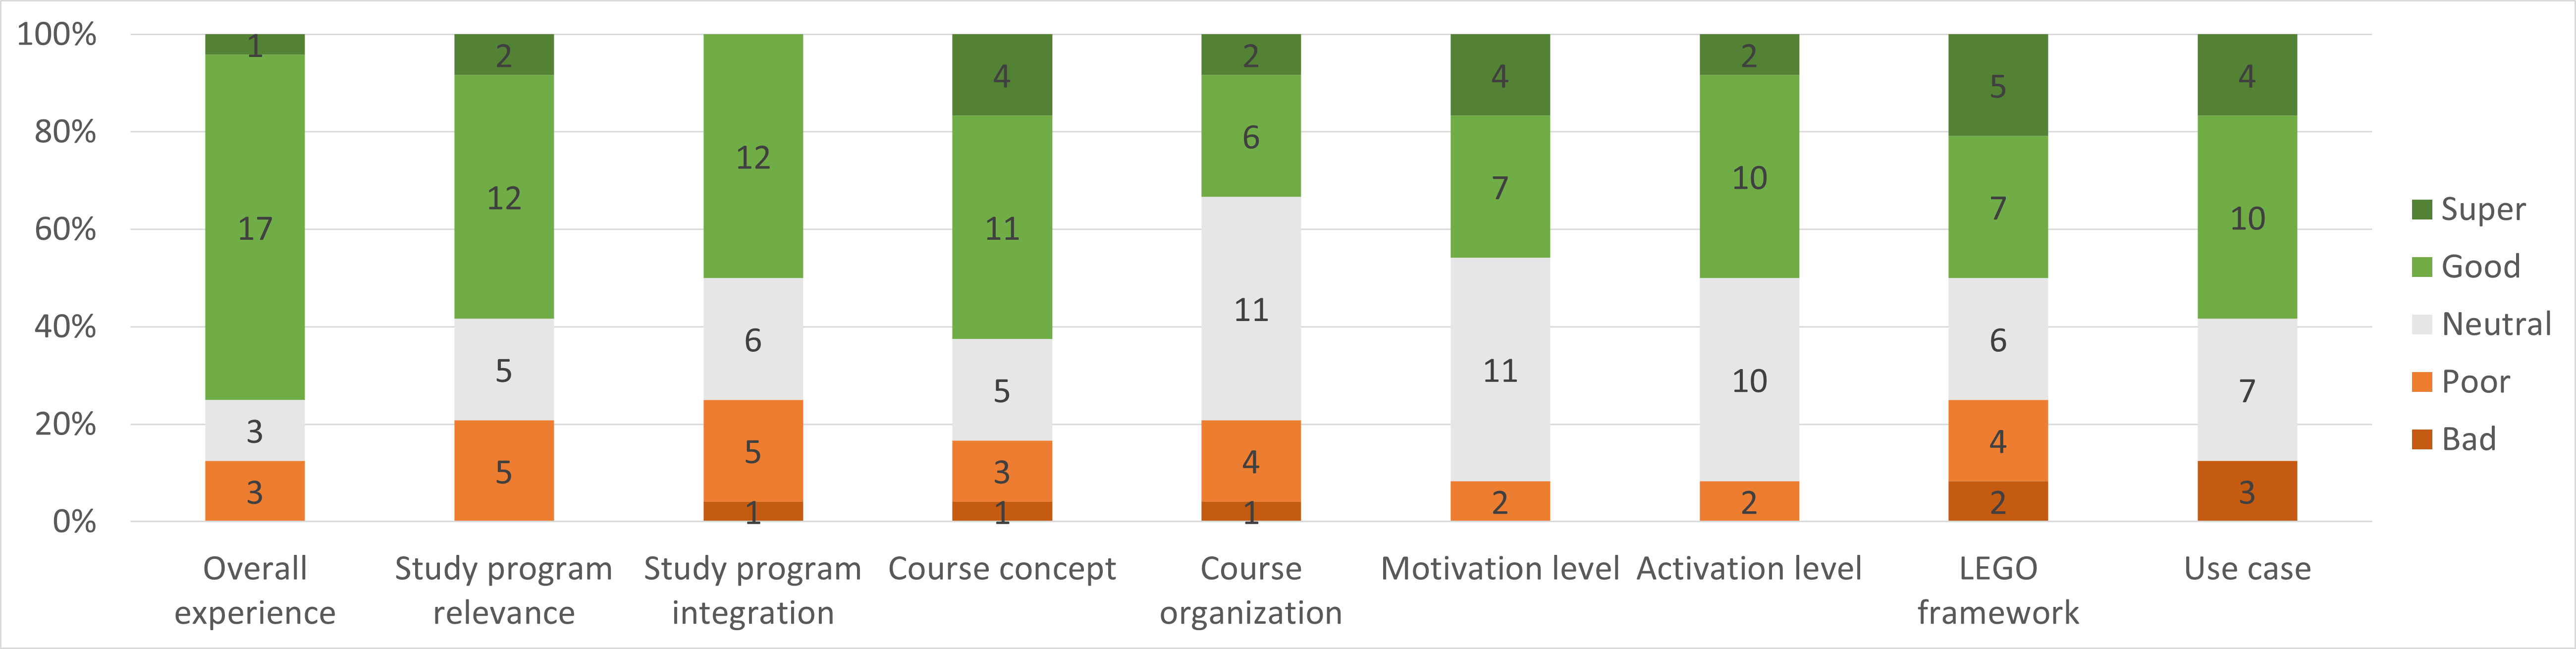
\includegraphics[width=\textwidth]{./diagrams/after-general.png}
    \caption{Summary of general learning experience during the course.}
    \label{fig:after-general}
\end{figure}

Then, Figure~\ref{fig:after-knowledge} summarizes the results of the assessment of the learning experience in different knowledge areas.
In particular, we assessed the learning experience the areas such as project management, agile methodology, product design, requirements engineering, computer-aided design, computer simulation, digital collaboration, and interdisciplinary collaboration.
Again the learning experience shows a positive tendency in all knowledge areas with product design, requirements engineering, and digital collaboration being among the best.
On the other hand, one can see potential for improvement in areas such as project management, agile methodology, computer-aided design, and systems engineering.

\begin{figure}[htbp]
    \centering
    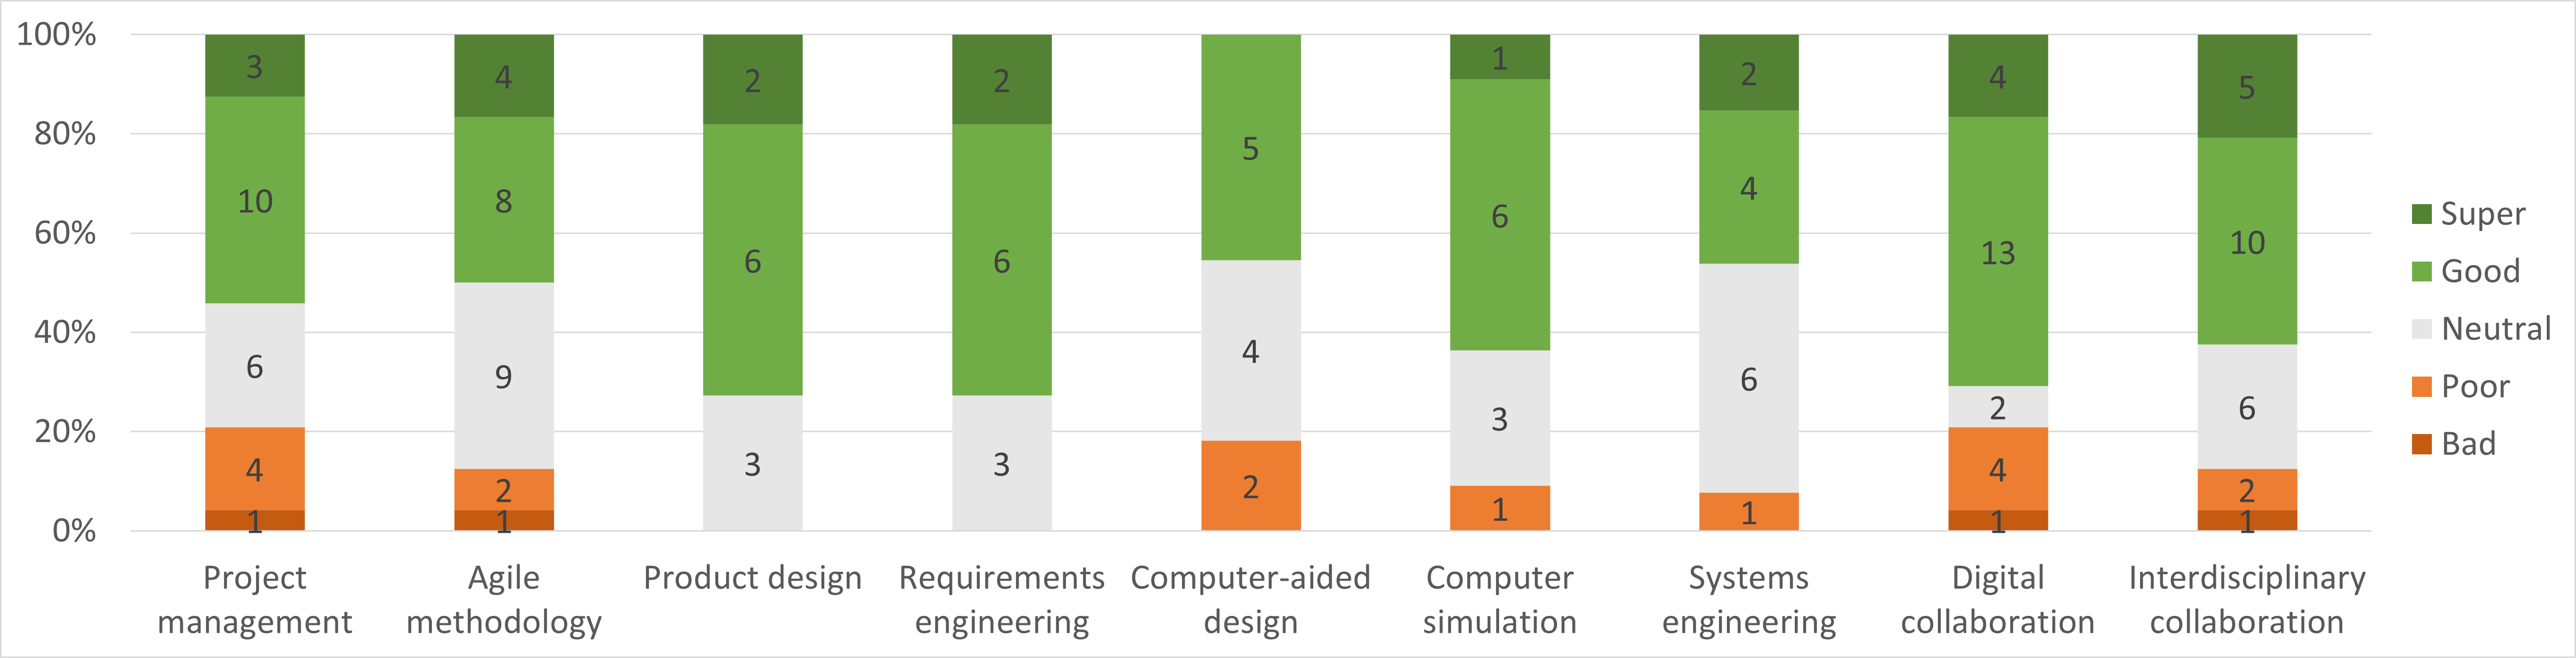
\includegraphics[width=\textwidth]{./diagrams/after-knowledge.png}
    \caption{Summary of learning experience in different knowledge areas.}
    \label{fig:after-knowledge}
\end{figure}

Finally, Figure~\ref{fig:after-software} summarizes the results of the assessment of the learning experience with different software tools.
In particular, the section of the questionnaire included the suitability, the usability, and the stability of the software tools CADdrive as the underlying collaboration platform, LeoCAD as the digital LEGO design tool, SimScale as a tool for finite element analysis and computational fluid dynamics, and OpenModelica as a tool for multi-physics simulation.
The results show a positive tendency for most software tools and characteristics including CADdrive at the forefront.
However, the results also reveal usability and stability issues with LeoCAD, which hinder the learning experience.

\begin{figure}[htbp]
    \centering
    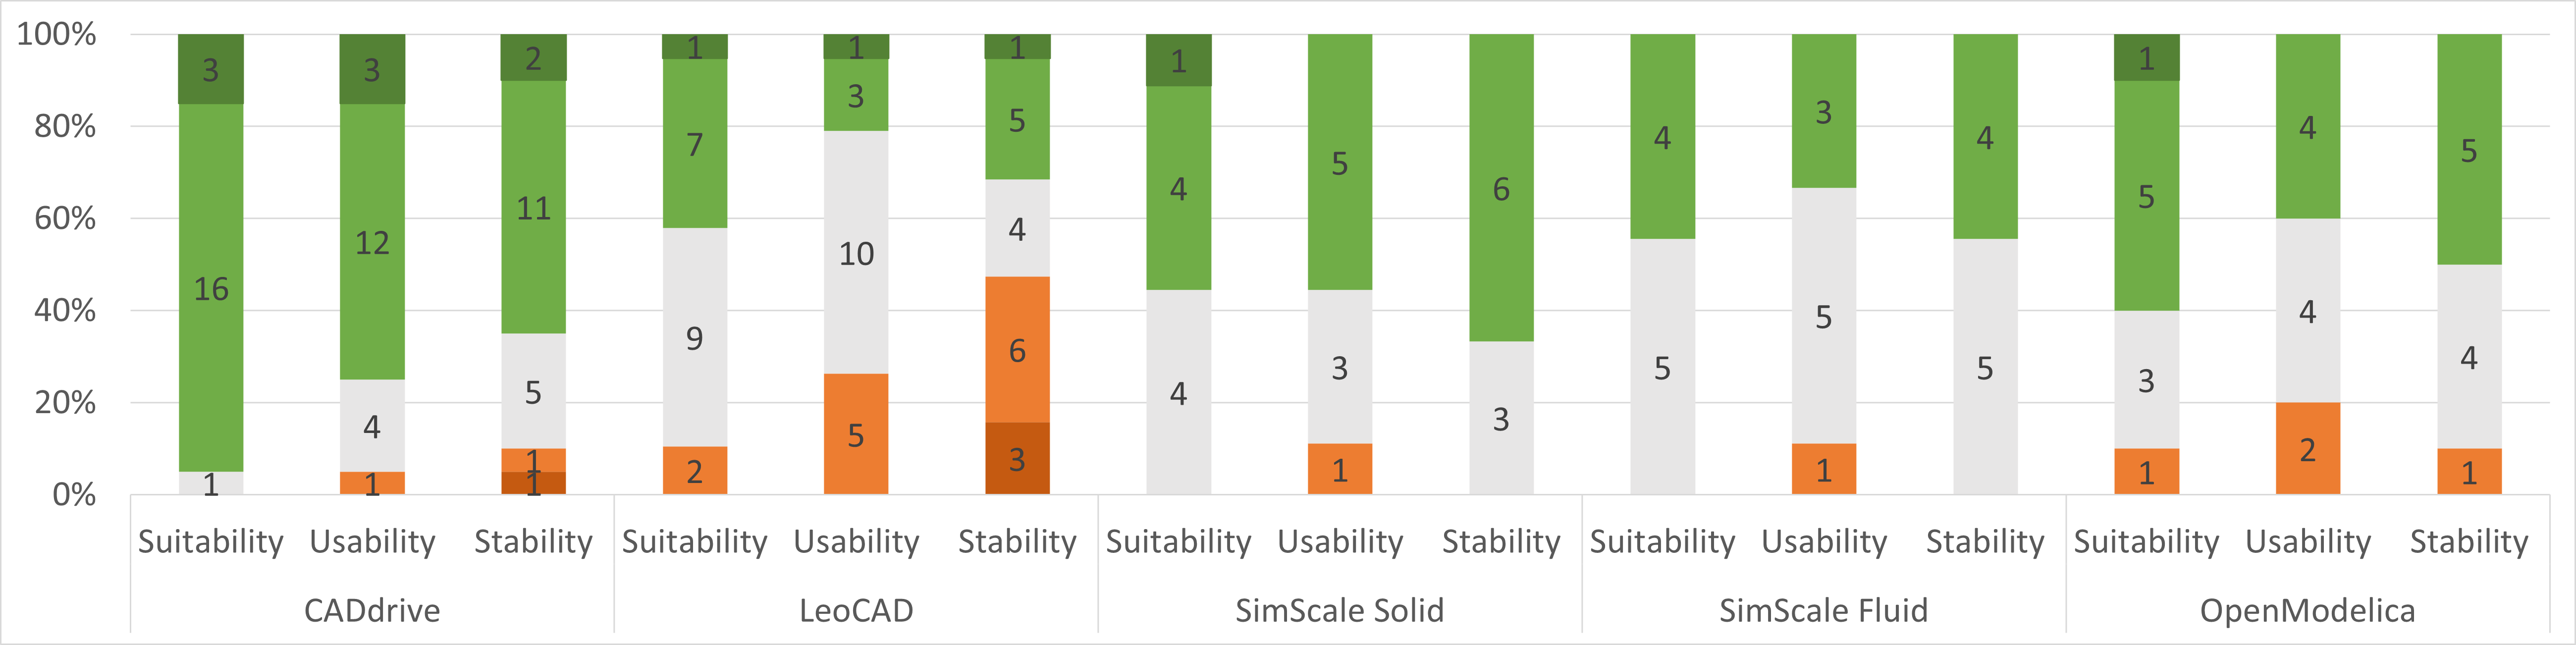
\includegraphics[width=\textwidth]{./diagrams/after-software.png}
    \caption{Summary of learning experience with the different software tools.}
    \label{fig:after-software}
\end{figure}

\subsubsection{Qualitative feedback}
\label{sec:qualitative}

The qualitative feedback section included three open questions about improvements of the course concept, improvement of the software tools, and miscellaneous feedback.
The feedback about the course concept mainly included requests for providing better course material with the course (e.g.\ about the theory of agile methodology and digital collaboration) as well as setting clear goals and communicating expectations for the outcomes of the product design and systems engineering projects.
The feedback about the software tools mainly included requests for CAD and simulation tool training prior to the course (e.g.\ multi-physics simulation with OpenModelica) as well as means for automatic up-scaling the brick resolution of LEGO models.
The LEGO brick resolution of the product and system models turned out to become an issue as the mechanical design teams progressed and started to add details, which were negelected initially.
Finally, the miscellaneous feedback mainly repeated the previous requests and included some positive statements about our innovative course format.

\section{Conclusions}
\label{sec:conclusion}

In the previous sections we first highlighted the need for innovation in engineering education with particular focus on collaboration, issues management, task scheduling, and early verification and validation.
Then, we presented our experiences with two Master-level courses on product design and systems engineering as well as a one-day workshop with children from high school including both quantitative and qualitative feedback from the participants.
In the following, we summarize our most important learnings from the previous experiments and sketch possible directions of future work in this field of research, development, and innovation.

\paragraph{Learnings}

While you possibly can learn many different things from the conducted experiments, here we concentrate on those learnings which we believe to be most generalizable and impactful for the product design and systems engineering community.
Furthermore, we decided to number the individual learnings for future reference and to enable more efficient and effective discussios around the underlying principles and mechanisms of design and engineering education.
Also, with each learning we include a short discussion of possible threats to validity, which are inherent with any scientific research study and the employed research methods.

\begin{description}
    \item[Learning 1]
    Overall, the two courses on product design (with simulation-based verification) and systems engineering (with mechanical, electrical, and logical design as well as review-based validation) using online collaboration tools such as CADdrive and digital LEGO design tools such as LeoCAD seem to be well suited for training Master students with different educational and professional backgrounds in a number of knowledge areas. Most prominently, the courses seem to foster learning in areas such as digital and interdisciplinary collaboration (i.e.\ team work) as well as product design and requirements engineering with relatively high levels of student motivation and activation.
    \item[Learning 2]
    Most Master students rated the digital LEGO framework as a viable foundation for such courses and learning experiences, but the opinions seem to be more controversial on this topic.
    When looking closer at the evaluation results, one can observe that the participants of the product design course (i.e.\ the glasshouse case) consistently preferred the digital LEGO framework, while the participants of the systems engineering course (i.e.\ the paper folding machine case) preferred using classical CAD instead.
    Two possible explanation are that the two cases are not equally well suited for the LEGO framework and that the systems engineering group faced more issues with LeoCAD due to model complexity.
    \item[Learning 3]
    The evaluation results also show that both the overall learning experience as well as the learning experience in the different knowledge areas still can be improved.
    When looking at the overall learning experience, the organization of the two courses seems to be the most effective lever for improving the course ratings.
    This impression can be confirmed when looking closer at the qualitative feedback showing mutliple requests for better course material as well as clearer definition of goals and expectations.
    We expect that additional course material with relevant theoretical inputs probably also helps improving the learning experience in the respective knowledge areas (e.g.\ agile methodology).
    \item[Learning 4]
    Finally, the work results as well as the informal feedback of the KunderUni workshop showed us, that our workshop format based on online collaboration platforms such as CADdrive and the digital LEGO framework are well suited for inspiring high school children for design and engineering topics.
    However, due to time limitations the workshop only covered digital LEGO design as well as version management (mastered by all teams) and component integration (mastered by three out of nine teams).
    We are confident, that with more time and proper training/tooling we can also cover topics such as requirements analysis, issue management, task scheduling, and simulation-based verification.
\end{description}

\paragraph{Outlook}

To advance the field of product design and systems engineering education even further, we currently work on several topics:
First we work on better CAD support for the digital LEGO framework to avoid the usability and stability issues experienced during our experiments.
Second we work on integrating classical mechanical and electrical CAD tools and their models into CADdrive to improve the learning experience of groups with stronger prior CAD knowledge.
And third, we work on adding explicit support for requirements management, systems architecture (including decomposition and interfacing), and computer simulation to improve the learning experience in these domains as well.

Beyond that we plan to extend the platform capabilities towards mechatronic product line engineering as explained by \cite{Michalek_2011}.
We believe that proper training concepts for product line engineering represent the next frontier, that we need to master in academic education so that our companies can benefit from these skills in the future and build larger varieties of products more efficiently and effectively.
Consequently, we need to add concepts such as product platforms, module repositories, interface compatibilities, and configuration models to CADdrive.
Furthermore, we need to redesign our courses to cover these topics in the course material as well as the cases considered during practical exercises.

\begin{Backmatter}

\bibliography{main}
\bibliographystyle{plainnat}

\end{Backmatter}

\end{document}